\documentclass{article}
\title{\textbf{3. MĚŘENÍ NA NAPĚŤOVÉM DĚLIČI}}
\author{Tomáš Kysela}
\date{21/2/2022}

\addtolength{\topmargin}{-3cm}
\addtolength{\textheight}{3cm}

\usepackage[czech]{babel}
\usepackage{graphicx}
\usepackage{circuitikz}
\usepackage{amsmath}
\usepackage{subcaption}
\usepackage{pgfplots}
\usepackage{siunitx}
\sisetup{detect-all}

\makeatletter
\providecommand\add@text{}
\newcommand\tagaddtext[1]{%
	\gdef\add@text{#1\gdef\add@text{}}}%
\renewcommand\tagform@[1]{%
	\maketag@@@{\llap{\add@text\quad}(\ignorespaces#1\unskip\@@italiccorr)}%
}
\makeatother


\begin{document}
	
	\maketitle
	
	\section{Úkol měření}
	\begin{enumerate}
		\item Změřte výstupní napětí $U_2$ děliče sestaveného z deseti rezistorů stejné jmenovité hodnoty pro všechny dělicí poměry $d$, a to:
		\begin{enumerate}
			\item číslicovým voltmetrem
			\item magnetoelektrickým voltmetrem (na rozsahu $12 \si{\volt}$).
		\end{enumerate}
		Do společného grafu vyneste závislosti $U_2 /U_1 = f(d)$ a vysvětlete jejich rozdíly. Velikost napájecího napětí děliče $U_1 = 10 \si{\volt}$.
		
		\item Z naměřených hodnot vypočtěte výstupní odpor děliče $R_D$ pro zadaný dělicí poměr za předpokladu, že vstupní odpor číslicového voltmetru se blíží k nekonečnu.
		
		\item Vypočtěte \textbf{rozšířenou nejistotu typu B} (koeficient rozšíření $k_r = 2$), s jakou jste určili výstupní odpor děliče $R_D$ za předpokladu, že vnitřní odpor magnetoelektrického voltmetru je definován s tolerancí $0.2\%$.
	\end{enumerate}
	\section{Schéma zapojení}
	\begin{figure}[htp]
		\centering
		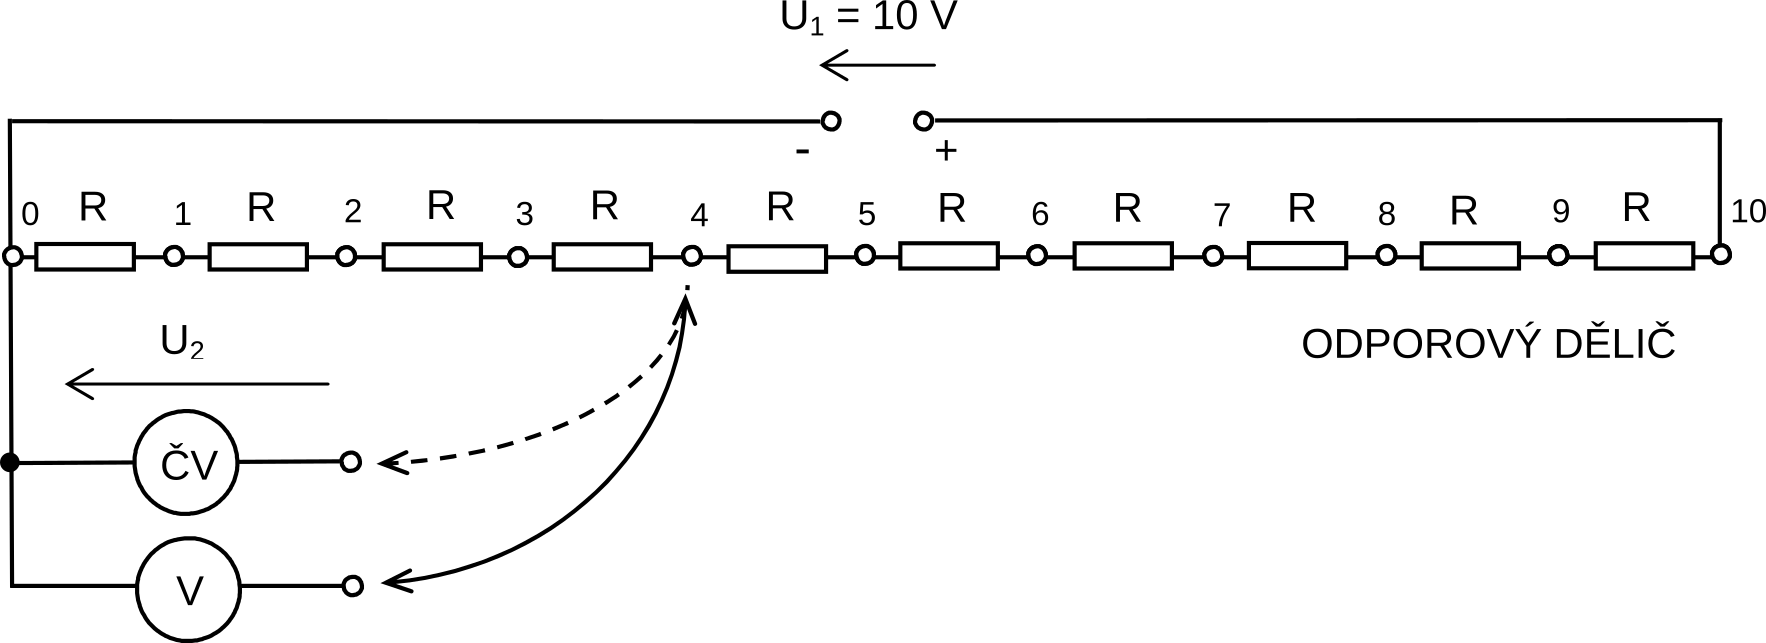
\includegraphics[scale=1.00]{LAB3.png}
		\caption{Schéma zapojení}
	\end{figure}
	\section{Soupis použitých přístrojů}
	\begin{tabular}{ll}
		V   & voltmetr magnetoelektrický, tř.přes. $0.5$, rozsah $12 V$, odpor $5000 \Omega/V$ \\
		ČV  & voltmetr číslicový, typ HP 34401A, $\pm 0,0035 \%$ údaje $\pm 0,0005 \%$ rozsahu \\
		U1  & zdroj stejnosměrného napětí, typ AGILENT E3640A                                  \\
		Př1 & odporový dělič
	\end{tabular}
	
	\section{Teoretický základ}
	
	Pokud měříme odporový dělič voltmetrem se srovnatelným vstupním odporem s výstupním odporem děliče, je hodnota $U_2$ menší než hodnota na prázdno $U_0$ (Obr 2a). Skutečný dělič napájený napětím $U_0$ zatížený voltmetrem se vstupním odporem $R_V$ (Obr 2b) lye nahradit Theveninovým náhradním obvodem (Obr 2c). Poté pro $U_2$ platí:
	\begin{equation}
		U_2 = U_0 \frac{R_v}{R_V + R_D} \tagaddtext{[\si{\volt}]}
	\end{equation}
	kde $R_D$ je výstupní odpor děliče.
	
	\begin{figure}[h]
		\centering
		\begin{subfigure}{0.4\textwidth}
			\begin{circuitikz}[european]
				\draw (1,-0.0) to[R,l_=$R_2$] (1,-2.0);
				\draw (1,-0.0) to[R,l=$R_1$] (1,2.0);
				\draw (1,2.0) to[short] (0,2.0);
				\draw (0,-1.0) to[short] (0,-2.0);
				\draw (0,-2.0) to[short] (1,-2.0);
				\draw (0,-1.0) to[esource,l=$U_1$] (0,1.0);
				\draw (0,1.0) to[short] (0,2.0);
				\draw (1,-0.0) to[short] (2,-0.0);
				\draw (1,-2.0) to[short] (2,-2.0);
				\draw (2, 0) to[open, v^>=$U_0$] (2,-2);
			\end{circuitikz}
			\caption{naprázdno}
		\end{subfigure}
		\begin{subfigure}{0.4\textwidth}
			\begin{circuitikz}[european]
				\draw (0,-1.0) to[esource,l=$U_1$] (0,1.0);
				\draw (1,2.0) to[R,l_=$R_1$] (1,-0.0);
				\draw (1,-0.0) to[R,l_=$R_2$] (1,-2.0);
				\draw (1,-2.0) to[short] (0,-2.0);
				\draw (0,-1.0) to[short] (0,-2.0);
				\draw (1,2.0) to[short] (0,2.0);
				\draw (0,2.0) to[short] (0,1.0);
				\draw (1,-0.0) to[short] (2,-0.0);
				\draw (1,-2.0) to[short] (2,-2.0);
				\draw (2,0.0) to[rmeter, t=V, v^>=$U_2$] (2,-2.0);
			\end{circuitikz}
			\caption{zatížený voltmetrem (odpor $R_V$)}
		\end{subfigure}
		\begin{subfigure}{0.4\textwidth}
			\begin{circuitikz}[european]
				\draw (0,1.0) to[R,l=$R_D$] (2,1.0);
				\draw (0,-1.0) to[esource,l=$U_1$] (0,1.0);
				\draw (2,1.0) to[rmeter, t=V, v^>=$U_2$] (2,-1.0);
				\draw (2,-1.0) to[short] (0,-1.0);
			\end{circuitikz}
			\caption{náhradní Théveninův obvod}
		\end{subfigure}
		\caption{Odporový dělič}
	\end{figure}
	
	Připojením voltmetru vzniká chyba, pro níž platí
	\begin{equation}
		\Delta U_{met}=U_2-U_0=U_0 \frac{R_V}{R_V+R_D} - U_0 = U_0 \frac{-R_D}{R_V + R_D } \tagaddtext{[\si{\ohm}]}
	\end{equation}
	
	Má-li voltmetr vstupní odpor mnohem vyšší, než je odpor děliče, pak je chyba metody zanedbatelná. Pro číslicový voltmetr se vstupním odporem $R_{CV}  \approx  10^9 \Omega$ tedy naměříme $U_0 \cong U_{2CV}$.
	
	Velikost výstupního odporu děliče můžeme zjistit buď z náhradního schématu 2c a vztahu (1),z něhož lze vyjádřit $R_D$:
	\begin{equation}
		R_D=\frac{R_V(U_{2CV}-U_2)}{U_2} = R_V(\frac{U_{2CV}}{U_2}-1) \tagaddtext{[\si{\ohm}]}
	\end{equation}
	Nebo pomocí proudu odporem $R_D$:
	\begin{equation}
		R_D=|\frac{U_{2CV}-U_2}{-I_2}| = R_V(\frac{U_{2CV}}{U_2}-1) \tagaddtext{[\si{\ohm}]}
	\end{equation}
	\subsection{Určení nejistoty měření výstupního odporu}
	
	Pokud jsou fluktuace měření zanedbatelné vůči přesnosti přístroje udávané výrobcem, je nejistota typu A zanedbatelná a napětí $U_{2CV}$ a $U_2$ potřebná pro výpočet odporu $R_D$ je třeba změřit pouze jednou. Jinak je třeba měření několikrát opakovat a z jejich aritmetických průměrů dostat nejistoty typu A.\\
	Lze předpokládat, že nejistoty typu A budou zanedbatelné a pro nejistotu $R_D$ tedy platí:
	\begin{equation}
		u_{RD}=\sqrt{(\frac{\partial R_D}{\partial U_{2CV}}u_{U2CV})^2+(\frac{\partial R_D}{\partial U_{2}}u_{U2})^2+(\frac{\partial R_D}{\partial R_{V}}u_{RV})^2} \tagaddtext{[\si{\ohm}]}
	\end{equation}
	
	\begin{equation}
		U_{RD} = u_{RD} k_r \tagaddtext{[\si{\ohm}]}
	\end{equation}
	
	\section{Naměřené hodnoty}
	\subsection{Naměřené hodnoty $U_2$ a $U_{2CV}$}
	\begin{tabular}{r||c|c||c|c}
		\textbf{Dělící poměr} & $U_2 [\si{\volt}]$ & $f(d)$ & $U_{2CV} [\si{\volt}]$ & $f_{CV}(d)$ \\ \hline \hline
		0.1 & 0.8 & 0.08 & 0.986 & 0.0986 \\ \hline
		0.2 & 1.5 & 0.15 & 1.981 & 0.1981 \\ \hline
		0.3 & 2.1 & 0.21 & 2.971 & 0.2971 \\ \hline
		0.4 & 2.7 & 0.27 & 3.982 & 0.3982 \\ \hline
		0.5 & 3.3 & 0.33 & 4.990 & 0.4990 \\ \hline
		0.6 & 4.1 & 0.41 & 5.976 & 0.5976 \\ \hline
		0.7 & 5.0 & 0.50 & 7.000 & 0.7000 \\ \hline
		0.8 & 6.1 & 0.61 & 8.001 & 0.8001 \\ \hline
		0.9 & 7.6 & 0.76 & 8.996 & 0.8996 \\ \hline
		1.0 & 10.0 & 1.00 & 9.996 & 0.9996
	\end{tabular}
	
	\begin{tikzpicture}
		\begin{axis}[
			title={Závislost $\frac{U_2}{U_1}$ $f(d)$, resp. $\frac{U_{2CV}}{U_1}$ ($f_{CV}(d)$)},
			xlabel={Dělící poměr [$\times10$]},
			ylabel={$f(d)$/$f_{CV}(d)$[$\times10$]},
			xmin=0, xmax=10.5,
			ymin=0, ymax=10.5,
			xtick={0,1,2,3,4,5,6,7,8,9,10},
			ytick={0,1,2,3,4,5,6,7,8,9,10},
			legend pos=north west,
			xmajorgrids=true,
			ymajorgrids=true,
			grid style=dotted,
			]
			
			\addplot[
			color=red,
			mark=*,
			]
			coordinates {
				(1,0.8)(2,1.5)(3,2.1)(4,2.7)(5,3.3)(6,4.1)(7,5.0)(8,6.1)(9,7.6)(10,10.0)
			};
			
			\addplot[
			color=blue,
			mark=*,
			]
			coordinates {
				(1,0.986)(2,1.981)(3,2.971)(4,3.982)(5,4.990)(6,5.976)(7,7.000)(8,8.001)(9,8.996)(10,9.996)
			};
			\legend{$\frac{U_2}{U_1}$,$\frac{U_{2CV}}{U_1}$}
			
		\end{axis}
	\end{tikzpicture}
	
	\subsection{Výpočet $R_D$}
	$$
	\begin{aligned}
		DP &= 0.2 \\
		R_1 &= 8R \\
		R_2 &= 2R \\
		R_D &= R_1 \parallel R_2 = \frac{R_1 R_2}{R_1 + R_2} = 1.6 R \\
		R_V &= 5000 \si{\ohm\per\volt} \\
		\\
		U_0 &= U_{2CV} = 1.981 \si{\volt} \\
		\\
		R_D &= R_V (\frac{U_{2CV}}{U_2}-1)=5000\si{\ohm}(\frac{1.981 \si{\volt}}{1.5 \si{\volt}}-1) = 5000 \si{\ohm} (1.321-1)=1605 \si{\ohm}\\
		R &= \frac{R_D}{1.6} = \frac{1605 \si{\ohm}}{1.6} = 1003.125 \si{\ohm}
	\end{aligned}
	$$
	
	\section{Výpočet nejistot}
	$$
	\begin{aligned}
		u_{2CV} &= \frac{\sigma_1 U_{2CV} + \sigma_2 M_{CV}}{100 \sqrt{3}} = \frac{\pm 0.0035 \% \cdot 1.981 \si{\volt} + \pm 0.0005 \% \cdot 10 \si{\volt}}{100 \sqrt{3}} = \pm 6.9 \cdot 10^{-5} \si{\volt} \\
		u_2 &= \frac{TP \cdot M}{100 \sqrt{3}} = \frac{0.5 \cdot 12 \si{\volt}}{100 \sqrt{3}} = \pm3.46 \cdot 10^{-2} \si{\volt} \\
		u_{RV} &= \frac{\sigma_{RV} R_V}{100 \sqrt{3}} = \frac{\pm 1 \% \cdot 5000 \si{\ohm\per\volt}}{100 \sqrt{3}} = \pm 28.87 \si{\ohm\per\volt} \\
		\\
		\frac{\partial R_D}{\partial U_{2CV}} &= \frac{R_V}{U_2} = \frac{5000 \si{\ohm\per\volt}}{1.5 \si{\volt}} = 3333.33 \si{\ohm\per\volt\squared} \\
		\frac{\partial R_D}{\partial U_2} &= -\frac{R_V U_{2CV}}{U_2} = -\frac{5000 \si{\ohm\per\volt} \cdot 1.981 \si{\volt}}{1.5 \si{\volt}} = -4402 \si{\ohm\per\volt} \\
		\frac{\partial R_D}{\partial R_V} &= \frac{U_{2CV} - U_2}{U_2} = \frac{1.981 \si{\volt} - 1.5 \si{\volt}}{1.5 \si{\volt}} = 0.32 \\
		\\
		u_{RD} &= \sqrt{(\frac{\partial R_D}{\partial U_{2CV}}u_{U2CV})^2+(\frac{\partial R_D}{\partial U_{2}}u_{U2})^2+(\frac{\partial R_D}{\partial R_{V}}u_{RV})^2} = \pm 153 \si{\ohm} \\
		\\
		U_{RD} &= u_{RD} k_r = \pm 153 \si{\ohm} \cdot 2 = \pm 306 \si{\ohm} \\
		U_{R} &= \frac{U_{RD}}{1.6} = \pm 191.25 \si{\ohm}
	\end{aligned}
	$$
	
	\section{Závěr}
	Určili jsme velikost vstupního odporu $R_D$ a to $1605 \pm 306 \si{\ohm}$ a velikost odporu $R$, což je $1003.125 \pm 191.250 \si{\ohm}$.
	
\end{document}